\documentclass{beamer}

\mode<presentation> {

%\usetheme{default}
%\usetheme{AnnArbor}
%\usetheme{Antibes}
%\usetheme{Bergen}
%\usetheme{Berkeley}
%\usetheme{Berlin}
%\usetheme{Boadilla}
%\usetheme{CambridgeUS}
%\usetheme{Copenhagen}
%\usetheme{Darmstadt}
%\usetheme{Dresden}
%\usetheme{Frankfurt}
%\usetheme{Goettingen}
%\usetheme{Hannover}
%\usetheme{Ilmenau}
%\usetheme{JuanLesPins}
%\usetheme{Luebeck}
\usetheme{Madrid}
%\usetheme{Malmoe}
%\usetheme{Marburg}
%\usetheme{Montpellier}
%\usetheme{PaloAlto}
%\usetheme{Pittsburgh}
%\usetheme{Rochester}
%\usetheme{Singapore}
%\usetheme{Szeged}
%\usetheme{Warsaw}


%\usecolortheme{albatross}
%\usecolortheme{beaver}
%\usecolortheme{beetle}
%\usecolortheme{crane}
%\usecolortheme{dolphin}
%\usecolortheme{dove}
%\usecolortheme{fly}
%\usecolortheme{lily}
%\usecolortheme{orchid}
%\usecolortheme{rose}
%\usecolortheme{seagull}
%\usecolortheme{seahorse}
%\usecolortheme{whale}
%\usecolortheme{wolverine}

%\setbeamertemplate{footline} % To remove the footer line in all slides uncomment this line
%\setbeamertemplate{footline}[page number] % To replace the footer line in all slides with a simple slide count uncomment this line

%\setbeamertemplate{navigation symbols}{} % To remove the navigation symbols from the bottom of all slides uncomment this line
}

\usepackage{graphicx} % Allows including images
\usepackage{booktabs} % Allows the use of \toprule, \midrule and \bottomrule in tables
\usepackage{amsfonts}
\usepackage{mathrsfs, bbold}
\usepackage{amsmath,amssymb,graphicx}
\usepackage{mathtools} % gather
\usepackage[export]{adjustbox} % right-aligned graphics

%----------------------------------------------------------------------------------------
%	TITLE PAGE
%----------------------------------------------------------------------------------------

\title["7"]{7: Evaluating, comparing and expanding models}

\author{Taylor} 
\institute[UVA] 
{
University of Virginia \\
\medskip
\textit{} 
}
\date{} 

\begin{document}
%----------------------------------------------------------------------------------------

\begin{frame}
\titlepage 
\end{frame}

%----------------------------------------------------------------------------------------
\begin{frame}
\frametitle{Introduction}

This chapter focuses mostly on quantifying a model's predictive capabilities for the purposes of model selection and expansion. 

\end{frame}

%----------------------------------------------------------------------------------------
\begin{frame}
\frametitle{New Notation!}

\begin{enumerate}
\item $f$ is the true model 
\item $y$ is the data we use to estimate our model
\item $\tilde{y}$ is the future (time series) or alternative (not time series) data that we test our predictions on
\item $p_{\text{post}}(\tilde{y}) = p(\tilde{y} \mid y )$
\item $p_{\text{post}}(\theta) = p(\theta \mid y)$
\item $E_{\text{post}}[ \cdot ] $ is taken with respect to $p(\theta \mid y)$
\end{enumerate}


\end{frame}


%----------------------------------------------------------------------------------------
\begin{frame}
\frametitle{Definitions}

A {\bf scoring rule/function} $S(p,\tilde{y})$ is a function that takes
\begin{enumerate}
\item the distribution you're using to forecast $p$ (ppd, or likelihood with estimated parameters), and 
\item a realized value $\tilde{y}$
\end{enumerate}
and then gives you a real-valued number/score/utility. Higher is better, although this convention isn't always followed in the literature.
\newline

Keep in mind that the realized value cannot be used to fit the data.
\end{frame}

%----------------------------------------------------------------------------------------
\begin{frame}
\frametitle{Examples}


Example: $S(p,\tilde{y}) = -(\tilde{y} - E_p[\tilde{y}])^2$
\newline


Example: $S(p,\tilde{y}) = \log p(\tilde{y})$
\newline


\end{frame}

%----------------------------------------------------------------------------------------
\begin{frame}
\frametitle{Definitions}

Future/unseen data is unknown, so we must take the expected score under the true distribution $f$:
$$
E_f[S(p,\tilde{y})].
$$

A scoring rule is {\bf proper} if the above expectation is minimized when $f = p$.
\newline

A scoring rule is {\bf local} if $S(p,\tilde{y})$ only depends on $p(\tilde{y})$ (don't care about events that didn't happen).
\newline

Note, when we are dealing with a logarithmic scoring rule, $E[-2\log p(\tilde{y})]$ is often called an {\bf information criterion.} The book switches back and forth between dealing with expected score, and information criteria. 

\end{frame}

%----------------------------------------------------------------------------------------
\begin{frame}
\frametitle{Examples}


Example: $S(p,\tilde{y}) = -(\tilde{y} - E_p[\tilde{y}])^2$ \\
Most common, perhaps not local or proper for non-Gaussian data.
\newline

Example: $S(p,\tilde{y}) = \log p(\tilde{y})$\\
Obviously local. Proper, too (homework question).


\end{frame}


%----------------------------------------------------------------------------------------
\begin{frame}
\frametitle{Problem}

% We may predict data with the ppd, or plug some point estimate $\hat{\theta}$ into the likelihood. 
% \newline

We are generally not able to evaluate the expectation because we don't know $f$. However, we may be able to wait for new out-of-sample data and use a Monte-Carlo approach:
\[
n^{-1}\sum_{i=1}^{n} S(p,\tilde{y}^i) \to E_f[S(p,\tilde{y})]
\]
as $n \to \infty$
\newline
\pause

If we can afford to wait for an infinite amount of data, though, what is the point of trying to predict it?

\end{frame}



%----------------------------------------------------------------------------------------
\begin{frame}
\frametitle{Problem}

NB: the textbook focuses on $S(p,\tilde{y}) = \log p(\tilde{y})$, and the data are iid (after conditioning on the parameter). They call the following quantity the ``elppd:"

\begin{block}{expected log pointwise predictive density}
\begin{align*}
E_f [\log p(\tilde{y})] &= E_f\left[\log \prod_i p(\tilde{y}_i) \right] \\
&= \sum_{i=1}^nE_f\left[ \log p(\tilde{y}_i) \right]
\end{align*}
\end{block}

\end{frame}

%----------------------------------------------------------------------------------------
\begin{frame}
\frametitle{Problem}

For the moment let's use $p(\tilde{y}) = p_{\text{post}}(\tilde{y})$
\newline

The ``elppd" is not obtainable because
\begin{enumerate}
\item you don't know $f$ (can't directly integrate)
\item you don't have $\tilde{y}$ (no Monte-Carlo)
\end{enumerate}
\pause

Using $y$ for $\tilde{y}$, we can come up with a rough elppd estimate called the ``lppd"
\begin{block}{log pointwise predictive density}
\[
\text{lppd} = \log p_{\text{post}}(y) = \sum_{i=1}^n \log p_{\text{post}}(y_i) 
\]
\end{block}



\end{frame}

%----------------------------------------------------------------------------------------
\begin{frame}
\frametitle{Problem}

There'a also the problem that arises where we cannot evaluate 
\[
p_{\text{post}}(y) = \int p(y \mid \theta) p(\theta \mid y) \text{d}\theta = E_{\text{post}}[p(y \mid \theta)]
\]

The ``computed lppd" again uses $y$ for $\tilde{y}$, but it also uses Monte-Carlo to sample from the posterior 
\begin{block}{log pointwise predictive density}
\[
\text{computed lppd} = \log \hat{p}_{\text{post}}(y) = \sum_{i=1}^n \log \left( \frac{1}{S} \sum_{j=1}^n p(y_i \mid \theta^j) \right) 
\]
\end{block}

-Biased and probably high variance, though.

\end{frame}



%----------------------------------------------------------------------------------------
\begin{frame}
\frametitle{Three problems}

Don't know $f$, don't want to wait for $\tilde{y}$...
\newline

and unfortunately, plugging the same data that we used for estimation into the predictive distribution might lead us to overfit because this strategy overestimates the average predictive score. What do we do?
\newline
\pause

However, we can get around this in two ways generally:
\begin{enumerate}
\item plug in the already-used $y$ data, but then add an extra penalty term (e.g. AIC, DIC, WAIC, etc.)
\item Cross-Validation: split the data $y$, many different ways, into a train and test set; estimate and evaluate on each split.
\end{enumerate}

\end{frame}

%----------------------------------------------------------------------------------------
\begin{frame}
\frametitle{Information Criteria}

{\bf AIC} stands for ``an information criterion" or ``Akaike's Information Criterion." Let $k$ be the number of parameters:
\newline

\[
\widehat{\text{elpd}}_{\text{AIC}} = \log p(y \mid \hat{\theta}_{\text{MLE}}) - \overbrace{k}^{\text{penalty}}
\]
or
\[
\text{AIC} = \underbrace{-2\log p(y \mid \hat{\theta}_{\text{MLE}})}_{\text{a deviance}} +2 k
\]

We estimate $\hat{\theta}_{\text{MLE}}$ using $y$, \*and\* we plug $y$ into the log likelihood. 

\end{frame}


%----------------------------------------------------------------------------------------
\begin{frame}
\frametitle{Information Criteria}

{\bf DIC} replaces the point estimate with $\hat{\theta}_{\text{Bayes}} = E[\theta \mid y]$, and replaces the penalty term with $p_{\text{DIC}}$
\newline

\[
\widehat{\text{elpd}}_{\text{DIC}} = \log p(y \mid \hat{\theta}_{\text{Bayes}}) - p_{\text{DIC}}
\]
or
\[
\text{DIC} = -2\log p(y \mid \hat{\theta}_{\text{Bayes}}) +2 p_{\text{DIC}}
\]

\end{frame}

%----------------------------------------------------------------------------------------
\begin{frame}
\frametitle{Information Criteria}

The book gives two ways to estimate $p_{\text{DIC}}$:

\begin{enumerate}
\item $p_{\text{DIC}} = 2\left(\log p(y \mid \hat{\theta}_{\text{Bayes}}) - E_{\text{post}}\left[ \log p(y \mid \theta) \right] \right)$
\item $p_{\text{DIC alt}} = 2 \operatorname{Var}_{\text{post}}\left[ \log p(y \mid \theta) \right]$
\end{enumerate}

Both of these can be approximated using samples from the posterior.

\end{frame}

%----------------------------------------------------------------------------------------
\begin{frame}
\frametitle{Information Criteria}

Motivation for $p_{\text{DIC}}$
\begin{align*}
&E_{\tilde{y}}\left[-2  \log p(\tilde{y} \mid \hat{\theta}_{\text{Bayes}})  \right] \\
&= - 2\log p(y \mid \hat{\theta}_{\text{Bayes}}) + E_{\tilde{y}}\left[  -2\log p(\tilde{y} \mid \hat{\theta}_{\text{Bayes}})  \right] + 2\log p(y \mid \hat{\theta}_{\text{Bayes}})\\
&\approx - 2\log p(y \mid \hat{\theta}_{\text{Bayes}}) +  E_{\theta \mid y}\left[ - 2 \log p(y \mid \theta) \right] + 2 \log p(y \mid \hat{\theta}_{\text{Bayes}} ) \\
&= - 2\log p(y \mid \hat{\theta}_{\text{Bayes}}) + p_{\text{DIC}}
\end{align*}


\end{frame}


%----------------------------------------------------------------------------------------
\begin{frame}
\frametitle{Information Criteria}

$p_{\text{WAIC}}$ either stands for ``widely applicable information criterion" or ``Watanabe-Akaike information criterion." 
\newline

The book refers to it as the most ``fully Bayesian" of the three, probably because it doesn't plug in point estimates into the likelihood instead of integrating.

\[
\widehat{\text{elppd}}_{\text{WAIC}} = \text{lppd} - p_{\text{WAIC}}
\]
or
\[
\text{WAIC} = -2\text{lppd} + 2 p_{\text{WAIC}}
\]

where $ \text{lppd} = \sum_{i=1}^n \log \left(\frac{1}{S}\sum_{s=1}^S p(y_i \mid \theta^s) \right)$

\end{frame}

%----------------------------------------------------------------------------------------
\begin{frame}
\frametitle{Information Criteria}

Two ways to estimate 

\begin{enumerate}
\item $p_{\text{WAIC 1}} = 2\left( \log p(y \mid y) - E_{\theta \mid y} \left\{  \log p(y \mid \theta) \right\} \right)$
\item $p_{\text{WAIC 2}} = \sum_{i=1}^n var_{\text{post}}(\log p(y_i \mid \theta))$
\end{enumerate}

Both of these can be approximated using samples from the posterior.

\end{frame}


%----------------------------------------------------------------------------------------
\begin{frame}
\frametitle{Information Criteria}

Motivation for $p_{\text{WAIC}}$:

\begin{align*}
&E_{\tilde{y}}\left[ -2  \log   p(\tilde{y} \mid y)  \right] \\
&E_{\tilde{y}}\left[ -2  \log  E_{\theta \mid y} ( p(\tilde{y} \mid \theta) ) \right] \\
&= - 2\log p(y \mid y) + 2\left( \log p(y \mid y) - E_{\tilde{y}}\left[  \log  E_{\theta \mid y} ( p(\tilde{y} \mid \theta) ) \right] \right) \\
&\approx - 2\log p(y \mid y) + 2\left( \log p(y \mid y) - E_{\tilde{y}}\left[   E_{\theta \mid y} ( \log  p(\tilde{y} \mid \theta) ) \right] \right) \\
&= - 2\log p(y \mid y) + 2\left( \log p(y \mid y) - E_{\theta \mid y}\left[   E_{\tilde{y}} (\log  p(\tilde{y} \mid \theta) ) \right] \right) \\
&\approx - 2\log p(y \mid y) + 2\left( \log p(y \mid y) - E_{\theta \mid y}\left[  \log   p(y \mid \theta)  \right] \right) \\
&= - 2\log p(y \mid y) + 2\left( \log \prod_i p(y_i \mid y) - E_{\theta \mid y}\left[  \log   \prod_i p(y_i \mid \theta)  \right] \right) \\
&= - 2\log p(y \mid y) + 2 \sum_i \left(  \log p(y_i \mid y) - E_{\theta \mid y}\left[ \log p(y_i \mid \theta)  \right] \right) \\
&= - 2\log p(y \mid y) + p_{\text{WAIC} 1}
\end{align*}



\end{frame}

%----------------------------------------------------------------------------------------
\begin{frame}
\frametitle{Cross-Validation}

To assess prediction performance, one may also use {\bf cross-validation}. Here the data is repeatedly partitioned into different training-set-test-set pairs (aka {\bf folds}).
\pause

\begin{enumerate}
\item The partitions are nonrandom, test sets are disjoint
\item for each split/estimation/prediction, we never use a data point twice
\item for each split/estimation/prediction, we lose parameter estimation accuracy because each training set is smaller than the full set
\item however, we get to average over many prediction scores, which reduces variance
\item there is still a bias that we have to estimate (but it's usually smaller than AIC/DIC/WAIC/etc.)
\item it can be computationally brutal to calculate for some models
\end{enumerate}
\pause


\includegraphics[width=50mm,right]{cv_logo.png}

The logo of this QA website illustrates the idea nicely!
\newline

\end{frame}

%----------------------------------------------------------------------------------------
\begin{frame}
\frametitle{Cross-Validation}


{\bf leave-one-out cross-validation} (loo-cv) is a special case where each test set is of size $1$.
\newline

This necessarily implies that each training set is of size $n-1$, and there are $n$ possible splits.
\newline

If this ends up being too computationally expensive, it is also possible to do {\bf $k$-fold cross-validation}, which selects $k$ splits/folds. This means the size of each test set is $n/k$, and the size of each training set is $n -n/k$

\end{frame}

%----------------------------------------------------------------------------------------
\begin{frame}
\frametitle{Cross-Validation Notation}

We only discuss loo-cv...
\newline

$p_{\text{post}(-i)}(y_i)$ is the prediction for the $i$th point, using the ppd, which uses the posterior distribution conditioning on all values of the data {\bf except the} $i$th
\newline
\pause

If this ppd isn't tractable, we can use draws from the posterior as follows:
\[
p_{\text{post}(-i)}(y_i) = \frac{1}{S}\sum_{s=1}^S p(y_i \mid \theta^s)
\]
where $\theta^s$ are draws from $p_{\text{post}(-i)}(\theta)$
\newline

\end{frame}

%----------------------------------------------------------------------------------------
\begin{frame}
\frametitle{Cross-Validation}


The Bayesian loo-cv estimate for out-of-sample predictive fit is 

\[
\text{lppd}_{\text{loo-cv}} = \sum_{i=1}^n \log p_{\text{post}(-i)}(y_i)
\]

There are also bias-corrected versions as well.

\end{frame}

%----------------------------------------------------------------------------------------
\begin{frame}
\frametitle{Bayes Factors}

{\bf Bayes factors} are another way to compare models, two at a time. You compare each model's prior predictive distribution/marginal likelihood/integrated likelihood/evidence:
\begin{block}{Bayes Factors}

\begin{align*}
B_{2,1} &= \frac{p(y \mid H_2)}{p(y \mid H_1)}\\
&= \frac{\int p(y \mid \theta_2, H_2)p(\theta_2 \mid H_2) \text{d}\theta_2}{\int p(y \mid \theta_1, H_1)p(\theta_1 \mid H_1) \text{d}\theta_1}
\end{align*}

assuming $0 < p(y \mid H_i) < \infty$
\end{block}

NB1: models do not have to be nested, and the parameters can be of varying dimension. \\
NB2: Unlike frequentist hypothesis testing, it measures the *strength* of one hypothesis over another.

\end{frame}

%----------------------------------------------------------------------------------------
\begin{frame}
\frametitle{Bayes Factors}

$B_{2,1} = \frac{p(y \mid H_2)}{p(y \mid H_1)}$

\begin{center}
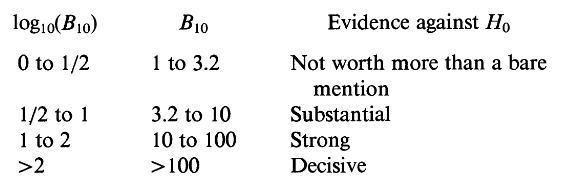
\includegraphics[width=80mm]{bf_scale.png}
\end{center}

From \url{http://www.andrew.cmu.edu/user/kk3n/simplicity/KassRaftery1995.pdf}

\end{frame}


%----------------------------------------------------------------------------------------
\begin{frame}
\frametitle{Bayes Factors}

The reason they call it a Bayes factor is because
\[
\text{posterior odds} = \text{Bayes factor} \times \text{prior odds}
\]
\pause

\begin{align*}
\text{posterior odds} &= \frac{p(H_2 \mid y)}{p(H_1 \mid y)} \\
&= \frac{p(y \mid H_2)p(H_2) / p(y)}{p(y \mid H_1)p(H_1) / p(y)} \tag{Bayes rule} \\
&= \frac{p(y \mid H_2)}{p(y \mid H_1)} \frac{p(H_2)}{p(H_1)} \\
&= \text{Bayes factor} \times \text{prior odds}
\end{align*}



\end{frame}


%----------------------------------------------------------------------------------------
\begin{frame}
\frametitle{Bayes Factors}

You should not use improper priors when you calculate Bayes factors because
\[
p(y \mid H_1) = \int p(y \mid \theta_1, H_1)p(\theta_1 \mid H_1) \text{d}\theta_1
\]
is not a density (homework question), and the normalizing constant will be ambiguous.

\end{frame}

%----------------------------------------------------------------------------------------
\begin{frame}
\frametitle{Bayes Factors}

Even noninformative proper priors can be ``biased" towards one of the hypotheses. 
\newline

% Consider HW question on page 194. 
% \newline

Consider the following example of the {\bf Jeffreys-Lindley's paradox}: 
\begin{enumerate}
\item under $H_1$: $\theta = 0$ with prior probability $1$
\item $p(\bar{y} \mid H_1)  = (2\pi)^{-n/2}n^{n/2} \exp\left[-\frac{n}{2}\bar{y}^2 \right]$
\item under $H_2$: $p(\theta) = N(0,\tau^2)$
\item $p(\bar{y} \mid H_2) = \int p(\bar{y} \mid \theta, H_2)p(\theta \mid H_2)\text{d}\theta = [2\pi(\tau^2 + n^{-1})]^{-n/2} \exp\left[-\frac{1}{2(\tau^2 + n^{-1})}\bar{y}^2 \right]$
\end{enumerate}
so
\[
B_{1,2} = (n\tau^2 + 1)^{1/2} \exp\left[-\frac{\bar{y}^2}{2}\left(n - \frac{1}{(\tau^2 + n^{-1})}\right) \right]
\]

\end{frame}

%----------------------------------------------------------------------------------------
\begin{frame}[fragile]
\frametitle{Bayes Factors: The Jeffreys-Lindley's paradox}

Say $\bar{y} = 1.5$ and $n = 10$. Then our p-value for the null is $2.101436e-06$, but 
\begin{center}
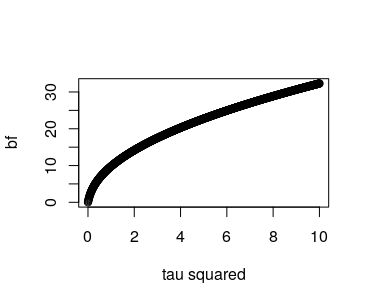
\includegraphics[width=75mm]{jf_paradox.png}
\end{center}

Different decisions based on whether we are frequentist or Bayesian?!

% \begin{verbatim}
% n <- 10
% ybar <- 1.5
% freq_test_stat <- sqrt(n)*ybar
% 2*pnorm(-abs(freq_test_stat))
% bf <- function(tausq) { 
%   (n*tausq + 1)^(1/2)*exp( -(ybar^2/2 ))*( n - 1 / (tausq + 1/n) ) 
% }
% tausq_grid <- seq(0,10, .01)
% plot(tausq_grid, bf(tausq_grid), xlab = "tau squared", ylab = "bf")
% \end{verbatim}



\end{frame}

%----------------------------------------------------------------------------------------
\begin{frame}
\frametitle{Bayes Factors}

If you can't derive $p(y \mid H_i)$, then it must be approximated. Noticing that the joint $p(y \mid \theta_i, H_i)p(\theta_i \mid H_i)$ is an unnormalized target, here is the justification behind importance sampling:

\begin{align*}
p(y \mid H_i) &= \int p(y \mid \theta_i, H_i)p(\theta_i \mid H_i) \text{d}\theta_i \\
&= \int \frac{p(y \mid \theta_i, H_i)p(\theta_i \mid H_i)}{q(\theta_i)}q(\theta_i) \text{d}\theta_i \\
&\leftarrow \sum_{s=1}^n \frac{p(y \mid \theta^s_i, H_i)p(\theta^s_i \mid H_i)}{q(\theta^s_i)}
\end{align*}

where $\theta^s_i \sim q(\theta_i)$.
\newline

Importance sampling will be discussed further in chapter 10.
\end{frame}

%----------------------------------------------------------------------------------------
\begin{frame}
\frametitle{Bayes Factors and the ``Worst Monte Carlo Method Ever" }

One might tempted to use the posterior samples, too:

\begin{align*}
p(y \mid H_i)
&= \left[ \frac{1}{p(y \mid H_i)} \int p(\theta_i \mid  H_i) \text{d}\theta_i \right]^{-1} \\
&= \left[  \int \frac{p(y \mid \theta_i,  H_i)p(\theta_i \mid H_i)}{p(y \mid H_i) p(y \mid \theta_i, H_i) } \text{d}\theta_i \right]^{-1}\\
&= \left[  \int \frac{p(\theta_i\mid y,  H_i) }{p(y \mid \theta_i, H_i) } \text{d}\theta_i \right]^{-1} \\
& \leftarrow  \left[  \frac{1}{S}\sum_{s=1}^S\frac{1 }{p(y \mid \theta_i^s, H_i) } \right]^{-1}
\end{align*}

where $\theta^s_i \sim p(\theta_i\mid y,  H_i)$ are samples from the posterior. 
\newline

However, this estimator often has infinite variance. There are a number of adjustments to this approach. 
\end{frame}

%----------------------------------------------------------------------------------------
\begin{frame}
\frametitle{Bayes Factors}

Under certain conditions, the {\bf Bayesian Information Criterion} or {\bf Schwarz Information Criterion} approximates the log of integrated likelihood. 
\[
BIC(H_i) = \log p(y \mid \hat{\theta}, H_i) - k \log(n)
\]
where $n$ is the number of data points, and $k$ is the dimension of $\theta$.
\newline

NB: you don't even need to specify a prior.

\end{frame}


\end{document} 


